\documentclass[]{article}
\usepackage{lmodern}
\usepackage{amssymb,amsmath}
\usepackage{ifxetex,ifluatex}
\usepackage{fixltx2e} % provides \textsubscript
\ifnum 0\ifxetex 1\fi\ifluatex 1\fi=0 % if pdftex
  \usepackage[T1]{fontenc}
  \usepackage[utf8]{inputenc}
\else % if luatex or xelatex
  \ifxetex
    \usepackage{mathspec}
  \else
    \usepackage{fontspec}
  \fi
  \defaultfontfeatures{Ligatures=TeX,Scale=MatchLowercase}
\fi
% use upquote if available, for straight quotes in verbatim environments
\IfFileExists{upquote.sty}{\usepackage{upquote}}{}
% use microtype if available
\IfFileExists{microtype.sty}{%
\usepackage{microtype}
\UseMicrotypeSet[protrusion]{basicmath} % disable protrusion for tt fonts
}{}
\usepackage{hyperref}
\hypersetup{unicode=true,
            pdfborder={0 0 0},
            breaklinks=true}
\urlstyle{same}  % don't use monospace font for urls
\usepackage{graphicx,grffile}
\makeatletter
\def\maxwidth{\ifdim\Gin@nat@width>\linewidth\linewidth\else\Gin@nat@width\fi}
\def\maxheight{\ifdim\Gin@nat@height>\textheight\textheight\else\Gin@nat@height\fi}
\makeatother
% Scale images if necessary, so that they will not overflow the page
% margins by default, and it is still possible to overwrite the defaults
% using explicit options in \includegraphics[width, height, ...]{}
\setkeys{Gin}{width=\maxwidth,height=\maxheight,keepaspectratio}
\IfFileExists{parskip.sty}{%
\usepackage{parskip}
}{% else
\setlength{\parindent}{0pt}
\setlength{\parskip}{6pt plus 2pt minus 1pt}
}
\setlength{\emergencystretch}{3em}  % prevent overfull lines
\providecommand{\tightlist}{%
  \setlength{\itemsep}{0pt}\setlength{\parskip}{0pt}}
\setcounter{secnumdepth}{0}
% Redefines (sub)paragraphs to behave more like sections
\ifx\paragraph\undefined\else
\let\oldparagraph\paragraph
\renewcommand{\paragraph}[1]{\oldparagraph{#1}\mbox{}}
\fi
\ifx\subparagraph\undefined\else
\let\oldsubparagraph\subparagraph
\renewcommand{\subparagraph}[1]{\oldsubparagraph{#1}\mbox{}}
\fi

\title{OER & Nutzung von PanDoc}
\author{Engelbert Niehaus}
\date{}

\begin{document}
\maketitle

{
\setcounter{tocdepth}{3}
\tableofcontents
}
\subsection{Wiki-Formate als
Datensenken}\label{wiki-formate-als-datensenken}

WikiMedia-Syntax wird als Format in

\begin{itemize}
\tightlist
\item
  Wikipedia
\item
  Wikiversity (OER)
\item
  OLAT (closed Doc Development)
\item
  ....
\end{itemize}

verwendet.

\subsection{WikiMedia-Konzept}\label{wikimedia-konzept}

\begin{itemize}
\tightlist
\item
  Offene kollaborative Inhaltsentwicklung
\item
  Versionierung der Inhalte
\item
  Diskussionsseiten jeweils zu allen Inhalten
\item
  Qualtitätsicherung mit externer Github-Versionierung und Querverweis
  zu Wiki-Referenz
\end{itemize}

\subsection{Wikiversity und
Bildungsprozesse}\label{wikiversity-und-bildungsprozesse}

\begin{itemize}
\tightlist
\item
  Primary Education (Grundschulen)
\item
  Secondary Education (Weiterführende Schulen)
\item
  Tertiary Education (Universitäten)
\item
  Non-formal Education (Handwerkliche Techniken, Alltagswissen, ...)
\end{itemize}

\subsection{Aus Datensenken andere Formate
erzeugen}\label{aus-datensenken-andere-formate-erzeugen}

\begin{itemize}
\tightlist
\item
  Markdown
\item
  Präsentationen (RevealJS, DZSlides, LaTeX Beamer)
\item
  LibreOffice-Dokumente mit Style-Templates,
\item
  Microsoft Office-Dokumente mit Style-Templates,
\item
  LaTeX-Dokumente,
\item
  PDF, ...
\end{itemize}

\subsection{PanDoc Electron}\label{pandoc-electron}

\begin{figure}[htbp]
\centering
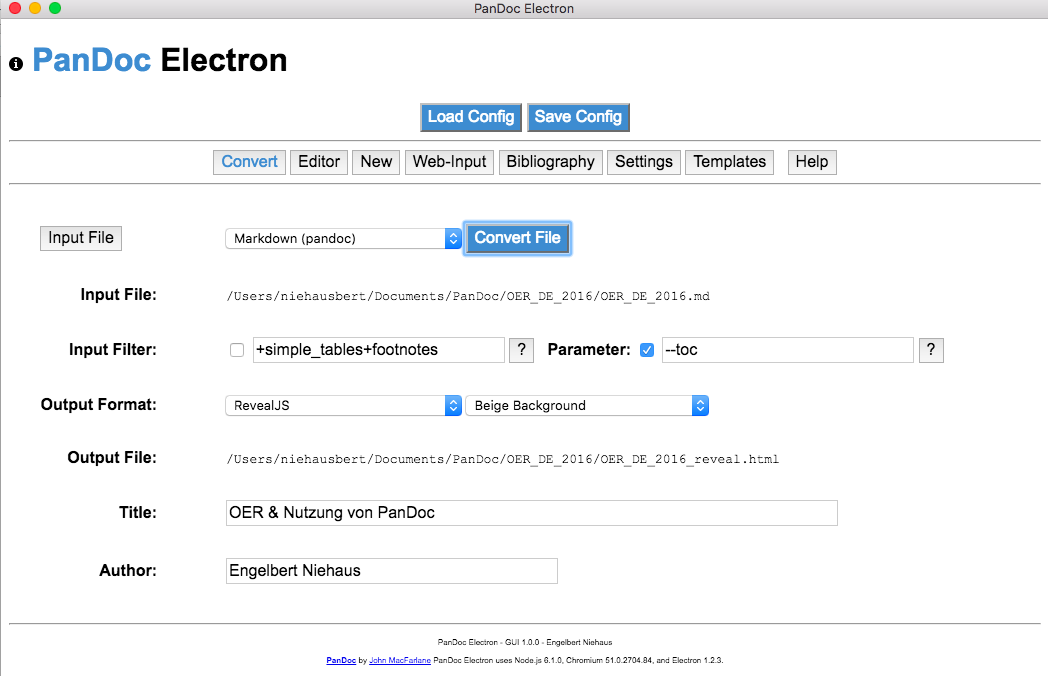
\includegraphics[width=7.29167in]{./images/PanDocElectronMain.png}
\caption{}
\end{figure}

\subsection{PanDoc Electron}\label{pandoc-electron-1}

\begin{figure}[htbp]
\centering
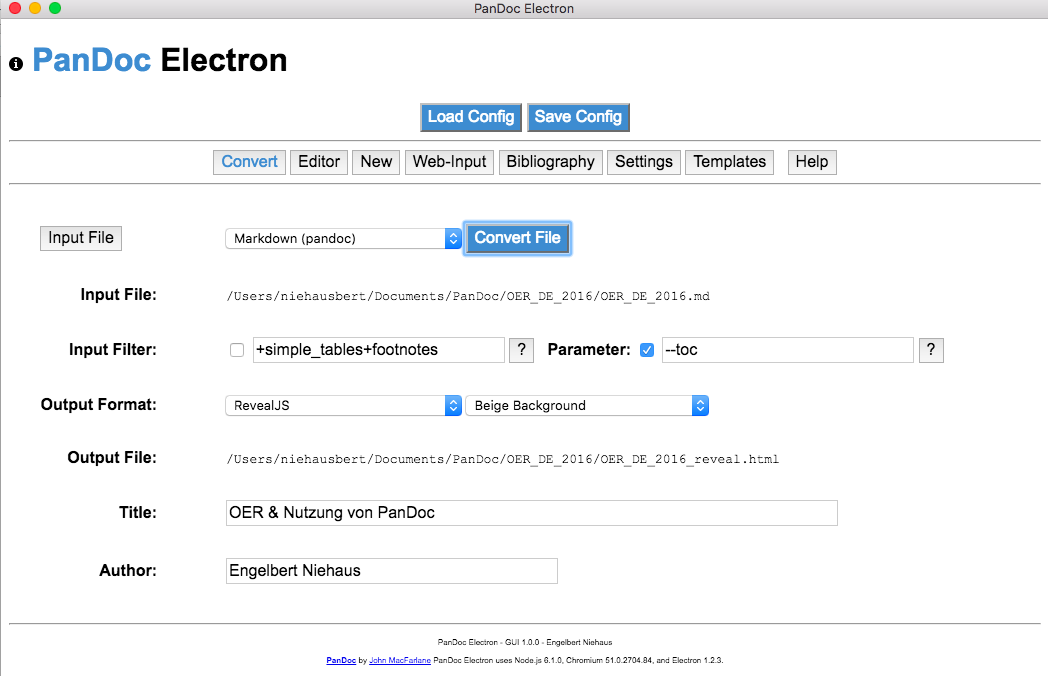
\includegraphics[width=2.60417in]{./images/PanDocElectronMain.png}
\caption{}
\end{figure}

\begin{itemize}
\tightlist
\item
  \textbf{Electron} = Browser mit vollem Zugriff auf das Dateisystem
\item
  \textbf{Download (PanDocElectron):}
  \href{http://niebert.github.io/PanDocElectron}{\url{http://niebert.github.io/PanDocElectron}}
\end{itemize}

\subsection{Reveal-Präsentationen}\label{reveal-pruxe4sentationen}

\begin{itemize}
\tightlist
\item
  In Standard
  \href{https://github.com/hakimel/reveal.js}{reveal.js}-Präsentationen
  werden mathematische Formel mit MathJax erzeugt.
\item
  Eingabeformate LaTeX (und ASCII-MathI)
\item
  URL: \url{https://github.com/mathjax/MathJax}
\item
  Homepage: \url{http://www.mathjax.org}
\end{itemize}

\subsection{Mathemtatik}\label{mathemtatik}

\begin{itemize}
\tightlist
\item
  z.B. Taylorentwickung
  \(f(x)=\sum_{n=0}^\infty\frac{f^{(n)}(a)}{n!}(x-a)^n\)\\
\end{itemize}

Abgesetzte mathematische Formeln
\(\displaystyle  \left( \sum_{k=1}^n a_k b_k \right)^2 \leq \left( \sum_{k=1}^n a_k^2 \right) \left( \sum_{k=1}^n b_k^2 \right)\)

\begin{itemize}
\tightlist
\item
  Grundlage LaTeX with in WikiMedia, MathJax, ... unterstützt
\end{itemize}

\subsection{Audio Video}\label{audio-video}

\begin{itemize}
\tightlist
\item
  Die Mediendateien werden in einen Unterverzeichnis der Projekte
  gespeichert \emph{/audio}, \emph{/video} and \emph{/images}
\item
  die Unterordner der Projekte Medien (Video, Audio, Images, ...),
\item
  insbesondere für Audiodateien zu Präsentationen \emph{audio1.mp3,
  audio2.mp3, ...}
\end{itemize}

\subsection{WikiMedia Quelle}\label{wikimedia-quelle}

\begin{figure}[htbp]
\centering
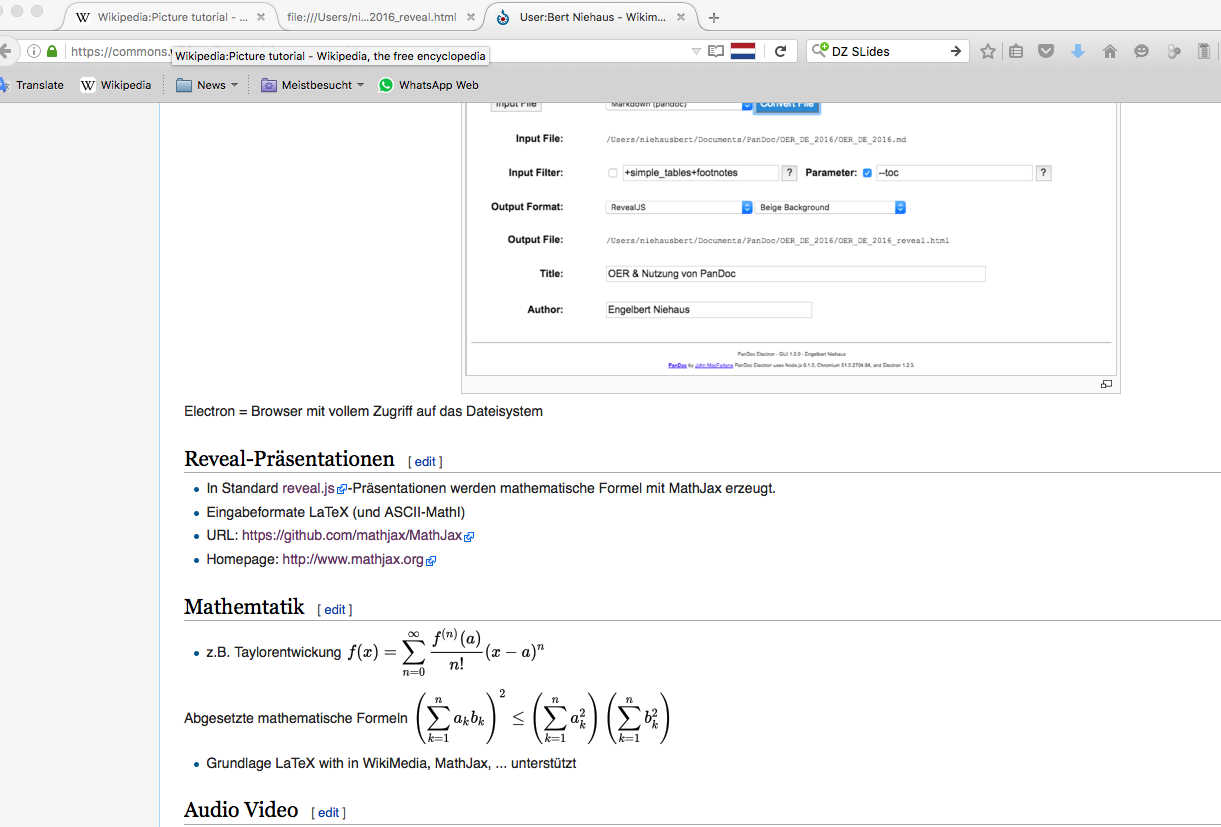
\includegraphics[width=6.77083in]{./images/PanDocWikiversity.png}
\caption{}
\end{figure}

\url{https://commons.wikimedia.org/wiki/User:Bert_Niehaus}

\subsection{PanDoc-Ausgabe:
LibreOffice}\label{pandoc-ausgabe-libreoffice}

\begin{figure}[htbp]
\centering
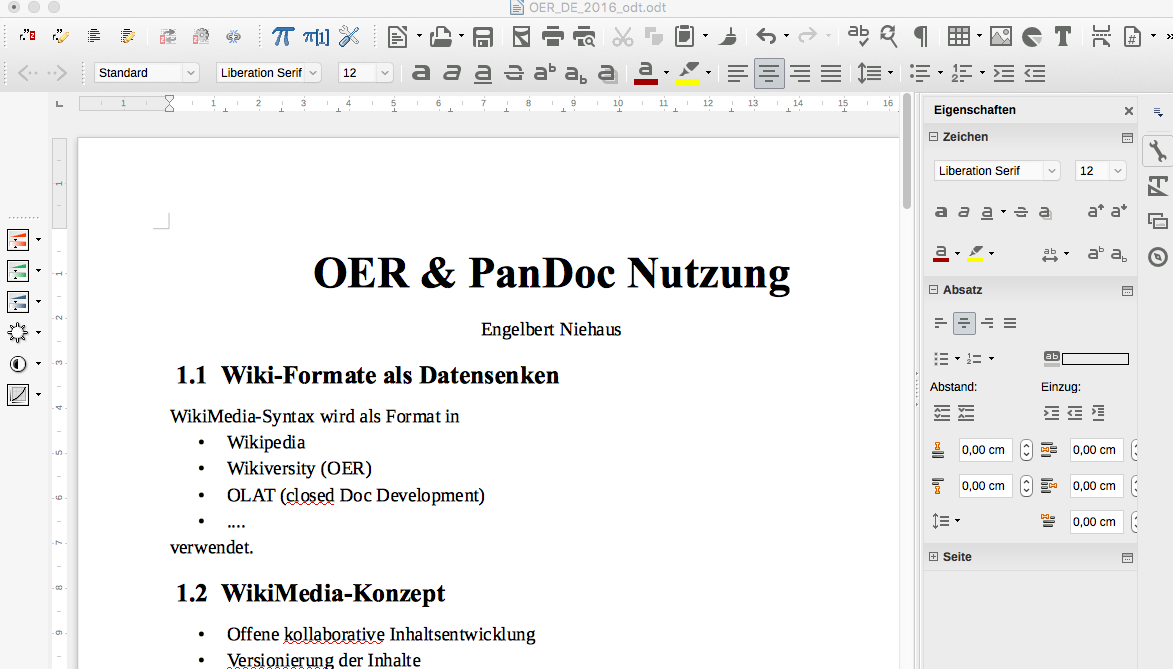
\includegraphics[width=6.77083in]{./images/PanDocLibreOffice1col.png}
\caption{}
\end{figure}

\subsection{PanDoc-Ausgabe: LibreOffice
Layout}\label{pandoc-ausgabe-libreoffice-layout}

\begin{figure}[htbp]
\centering
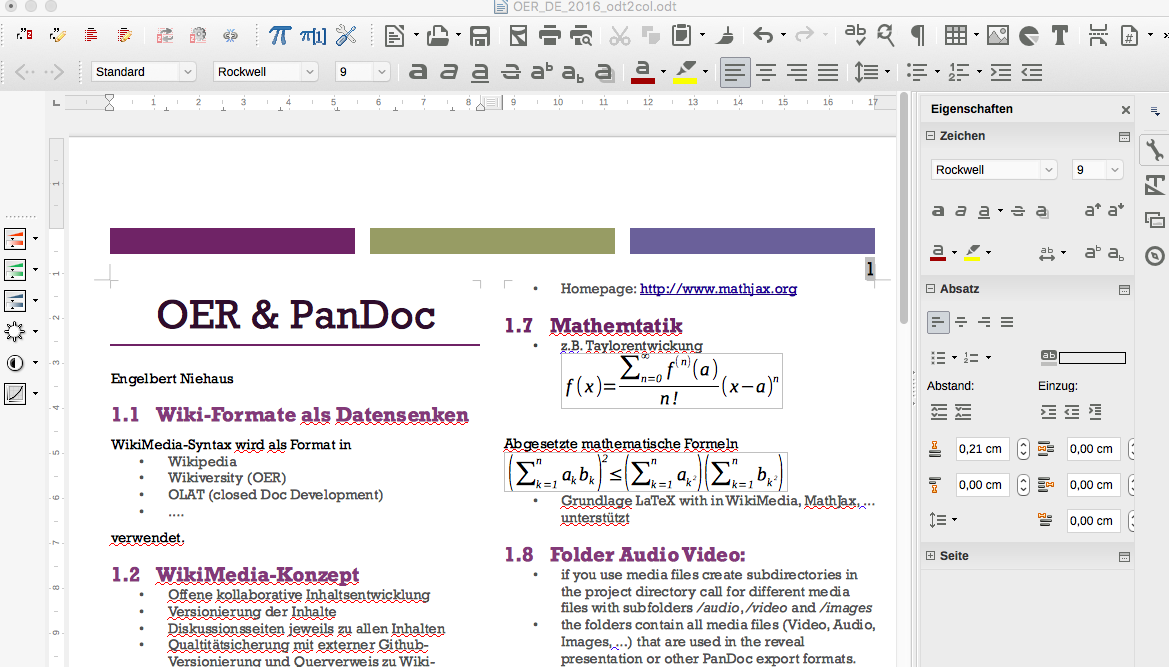
\includegraphics[width=6.77083in]{./images/PanDocLibreOffice2col.png}
\caption{}
\end{figure}

\subsection{PanDoc-Ausgabe: Word
Layout}\label{pandoc-ausgabe-word-layout}

\begin{figure}[htbp]
\centering
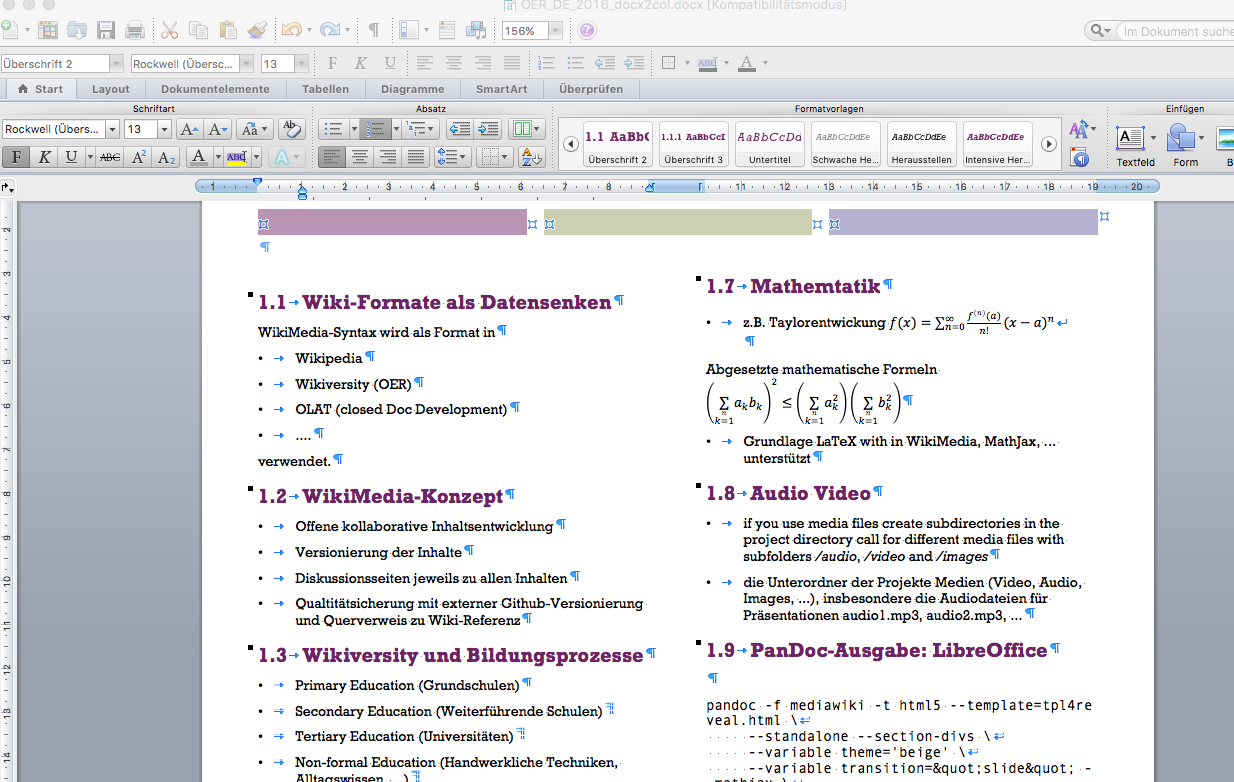
\includegraphics[width=6.77083in]{./images/PanDocWord2col.png}
\caption{}
\end{figure}

\subsection{PanDoc von der
Kommandozeile}\label{pandoc-von-der-kommandozeile}

\begin{verbatim}
pandoc -f mediawiki -t html5 --template=tpl4reveal.html \
     --standalone --section-divs \
     --variable theme='beige' \
     --variable transition=&quot;slide&quot; --mathjax \
     wikipedia.wiki -o wikipedia.html
\end{verbatim}

\subsection{GitHub: Versionierung einer
Qualitätssicherung}\label{github-versionierung-einer-qualituxe4tssicherung}

\begin{itemize}
\tightlist
\item
  GitHub zur Versionierung von Quelltexten (i.d. Programmcode)
\item
  für OER angewendet auf WikiMedia Quelltextes
\item
  Lese-Zugriff frei/offen
\item
  Schreibzugriff auf die Versionierung nur durch Gutachterteam
\item
  Gutachter-Innen nicht anonym
\end{itemize}

\subsection{Tutorials für Markdown \&
WikiMedia}\label{tutorials-fuxfcr-markdown-wikimedia}

\begin{itemize}
\tightlist
\item
  Tutorial Markdown \url{http://www.markdowntutorial.com}
\item
  Tutorial WikiMedia
  \url{https://en.wikipedia.org/wiki/Wikipedia:Tutorial}
\end{itemize}

\subsection{Zusammenfassung}\label{zusammenfassung}

\begin{itemize}
\tightlist
\item
  \textbf{Wikiversity:} Offene kollaborative Inhaltsentwicklung für OER
\item
  \textbf{Versionierung:} Inhalte werden versioniert inkl.
  Diskussionsseiten
\item
  \textbf{PanDoc(Electron):} Tools für Konvertierung der Inhalte in
  andere Formate
\item
  \textbf{Qualtitätsicherung:} Externer Github-Versionierung und
  Querverweis zu Wiki-Referenz
\end{itemize}

\end{document}
